% !TEX root = ./bursty_transcription.tex
\section{Bursty promoter models - generating function solutions and numerics}
\label{sec:gen_fcn_appdx}

\subsection{Constitutive promoter with bursts}

\subsubsection{From master equation to generating function}

The objective of this section is to write down the steady-state mRNA
distribution for model 5 in Figure~\ref{fig2:constit_cartoons}. Our claim is
that this model is rich enough that it can capture the expression pattern of
bacteria unregulated promoters regulated by the $\sigma_{70}$ sigma factor.
Figure~\ref{figS1:bursty_one_state} shows two different schematic
representations of the model. Figure~\ref{figS1:bursty_one_state}(A) shows the
promoter cartoon model with burst initiation rate $k_i$, mRNA degradation rate
$\gamma$, and mean burst size $b$. For our derivation of the chemical master
equation we will focus more on Figure~\ref{figS1:bursty_one_state}(B). This
representation is intended to highlight that bursty gene expression allows
transitions between mRNA count $m$ and $m'$ even with $m - m' > 1$.

\begin{figure}[h!]
\centering
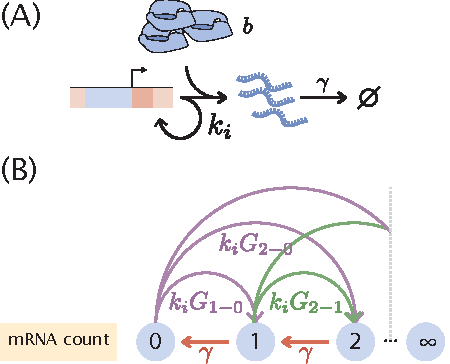
\includegraphics{../figures/si/figS0X_bursty_states.pdf}
\caption{
\textbf{Bursty transcription for unregulated promoter.}
(A) Schematic of the one-state bursty transcription model. Rate $k_i$ is the
bursty initiation rate, $\gamma$ is the mRNA degradation rate, and $b$ is the
mean burst size. (B) Schematic depiction of the mRNA count state transitions.
The model in (A) allows for transitions of $> 1$ mRNA counts with probability
$G_{m-m'}$.}
\label{figS1:bursty_one_state}
\end{figure}

To derive the master equation we begin by thinking the possible state
transitions to ``enter'' state $m$. There are two possible paths to jump from an
mRNA count $m' \neq m$ to a state $m$ in a small time window $\Delta t$:
\begin{enumerate}
        \item By degradation of a single mRNA, jumping from $m+1$ to $m$.
        \item By producing $m-m'$ mRNA for $m' \in \{0, 1, \ldots, m-1\}$.
\end{enumerate}
For the ``exit'' states from $m$ into $m' \neq m$ during a small time window
$\Delta t$ we also have two possibilities:
\begin{enumerate}
        \item By degradation of a single mRNA, jumping from $m$ to $m-1$.
        \item By producing $m'-m$ mRNA for $m'-m \in \{1, 2, \ldots\}$.
\end{enumerate}
This implies that the probability of having $m$ mRNA at time $t + \Delta t$ can
be written as
\begin{equation}
\begin{split}
p(m, t + \Delta t) = &p(m, t)
+ \overbrace{\gamma \Delta t (m + 1) p(m + 1, t)}^{m + 1 \rightarrow m}
- \overbrace{\gamma \Delta t m p(m, t)}^{m \rightarrow m - 1} \\
&+ \overbrace{k_i \Delta t \sum_{m'=0}^{m-1} G_{m-m'} p(m', t)}^
{m'\in \{0, 1, \ldots m-1\} \rightarrow m}
- \overbrace{k_i \Delta t \sum_{m'=m + 1}^{\infty} G_{m'-m} p(m, t)}^
{m \rightarrow m'\in \{m+1, m+2, \ldots\}},
\end{split}
\label{eq:si_master_deltat}
\end{equation}
where we indicate $G_{m'-m}$ as the probability of having a burst of size
$m'-m$. We suggestively use the letter $G$ as we will assume that these bursts
sizes are geometrically distributed with parameter $\theta$. This is written as
\begin{equation}
G_{k} = \theta (1 - \theta)^k\; \text{for } k \in \{0, 1, 2, \ldots \}.
\end{equation}
What this implies is that for a geometrically distributed burst size we have a
mean burst size $b$ of the form
\begin{equation}
b \equiv \left\langle m' - m \right\rangle 
= \sum_{k=0}^\infty k \theta (1 - \theta)^k = {1 - \theta \over \theta}.
\end{equation}

To clean up Equation~\ref{eq:si_master_deltat} we can send the first term on the
right hand side to the left, and divide both sides by $\Delta t$. Upon taking
the limit where $\Delta t \rightarrow 0$ we can write
\begin{equation}
{d \over dt}p(m, t) = (m + 1) \gamma p(m + 1, t)
- m \gamma p(m, t)
+ k_i \sum_{m'=0}^{m-1} G_{m-m'} p(m', t) 
- k_i \sum_{m'=m + 1}^{\infty} G_{m'-m} p(m, t).
\end{equation}
Furthermore, given that the timescale for this equation is set by the mRNA
degradation rate $\gamma$ we can divide both sides by this rate, obtaining
\begin{equation}
{d \over d\tau}p(m, \tau) = (m + 1) p(m + 1, \tau)
- m p(m, \tau)
+ \lambda \sum_{m'=0}^{m-1} G_{m-m'} p(m', \tau) 
- \lambda \sum_{m'=m + 1}^{\infty} G_{m'-m} p(m, \tau),
\label{eq:si_master_ode}
\end{equation}
where we defined $\tau \equiv t \times \gamma$, and $\lambda \equiv k_i/\gamma$.
The last term in Eq.~\ref{eq:si_master_ode} sums all burst sizes except for a 
burst of size zero. We can re-index the sum to include this term, obtaining
\begin{equation}
\lambda \sum_{m'=m + 1}^{\infty} G_{m'-m} p(m, \tau) = \lambda p(m, t) \left[
\underbrace{\sum_{m'=\textcolor{red}{m}}^{\infty}G_{m'-m}}
_{\text{re-index sum to include burst size zero}} -
\underbrace{G_0}_{\text{subtract extra added term}}\right].
\end{equation}
Given the normalization of the geometric distribution, adding the probability of
all possible burst sizes -- including size zero since we re-indexed the sum --
allows us to write
\begin{equation}
\sum_{m'=m}^{\infty}G_{m'-m} - G_0 = 1 - G_0.
\end{equation}
Substituting this into Eq.~\ref{eq:si_master_ode} results in
\begin{equation}
{d \over d\tau}p(m, \tau) = (m + 1) p(m + 1, \tau)
- m p(m, \tau)
+ \lambda \sum_{m'=0}^{m-1} G_{m-m'} p(m', \tau) 
- \lambda p(m, \tau) \left[ 1 - G_0 \right].
\label{eq:si_master_ode_2}
\end{equation}
To finally get at a more compact version of the equation notice that the third
term in Eq.~\ref{eq:si_master_ode_2} includes burst from size $m'-m = 1$ to size
$m' - m = m$. We can include the term $p(m, t) G_0$ in the sum which allows
bursts of size $m' - m = 0$. This results in our final form for the chemical
master equation
\begin{align}
{d \over d\tau}p(m, \tau) = 
(m + 1) p(m+1, \tau)
- m p(m, \tau) - 
\lambda p(m, \tau)
+ \lambda \sum_{m^\prime=0}^m G_{m-m^\prime} p(m^\prime, \tau).
\label{eq:si_master_unreg}
\end{align}

In order to solve Eq.~\ref{eq:si_master_unreg} we will use the generating
function method \mrm{reference?}. The probability generating function is defined
as
\begin{align}
F(z,t) = \sum_{m=0}^\infty z^m p(m,t),
\end{align}
where $z$ is just a dummy variable that will help us later on to obtain the
moments of the distribution. Applying $F(z, t)$ on both sides of 
Eq.~\ref{eq:si_master_unreg} results in
\begin{equation}
\sum_m z^m {d \over d\tau} p(m, \tau) = 
\sum_m z^m \left[ 
- m p(m, \tau) 
+ (m + 1) p(m + 1, \tau) 
+ \lambda \sum_{m' = 0}^m G_{m-m'} p(m', \tau) - \lambda p(m, \tau)
\right],
\end{equation}
where we use $\sum_m \equiv \sum_{m=0}^\infty$. We can distribute the sum and
use the definition of $F(z, t)$ to obtain
\begin{equation}
{d F(z, \tau) \over d\tau} =
- \sum_m z^m m p(m, \tau) +
+ \sum_m z^m (m + 1) p(m + 1, \tau)
+ \lambda \sum_m z^m \sum_{m'=0}^m G_{m-m'} p(m', \tau)
- \lambda F(z, \tau).
\label{eq:si_generating_01}
\end{equation}
We can make use of properties of the generating function to write everything in
terms of $F(z, \tau)$: the first term on the right hand side of
Eq.~\ref{eq:si_generating_01} can be rewritten as
\begin{align}
\sum_{m} z^{m} \cdot m \cdot p(m, \tau) &=
\sum_{m} z \frac{\partial z^{m}}{\partial z} p(m, \tau), \\
&=\sum_{m} z \frac{\partial}{\partial z}\left(z^{m} p(m, \tau)\right), \\
&=z \frac{\partial}{\partial z}\left(\sum_{m} z^{m} p(m, \tau)\right), \\
&= z {\partial F(z, \tau) \over \partial z}.
\end{align}
For the second term on the right hand side of Eq.~\ref{eq:si_generating_01} we
define $k \equiv m + 1$. This allows us to write
\begin{align}
\sum_{m=0}^{\infty} z^{m} \cdot(m+1) \cdot p(m+1, \tau) &=
\sum_{k=1}^{\infty} z^{k-1} \cdot k \cdot p(k, \tau), \\
&=z^{-1} \sum_{k=1}^{\infty} z^{k} \cdot k \cdot p(k, \tau), \\
&=z^{-1} \sum_{k=0}^{\infty} z^{k} \cdot k \cdot p(k, \tau), \\
&=z^{-1} \left(z \frac{\partial F(z)}{\partial z}\right), \\
&=\frac{\partial F(z)}{\partial z}.
\end{align}
The third term in Eq.~\ref{eq:si_generating_01} is the most trouble. The trick
is to reverse the default order of the sums as
\begin{equation}
\sum_{m=0}^{\infty} \sum_{m'=0}^{m} = \sum_{m'=0}^{\infty} \sum_{m=m'}^{\infty}.
\end{equation}
This results in
\begin{align}
\lambda \sum_m z^m \sum_{m'=0}^m G_{m-m'} p(m', \tau) =
\lambda \sum_{m'=0}^{\infty} \sum_{m=m'}^{\infty} z^m 
\theta (1 - \theta)^{m-m'} p(m', \tau),
\end{align}
where we also substituted the definition of the geometric distribution $G_{k} =
\theta (1 - \theta)^k$. Redistributing the sums we can write
\begin{align}
\lambda \sum_{m'=0}^{\infty} \sum_{m=m'}^{\infty} z^m 
\theta (1 - \theta)^{m-m'} p(m', \tau) = 
\lambda \theta \sum_{n=0}^{\infty}(1-\theta)^{m'} P(m', \tau) 
\sum_{m=m'}^{\infty} \left[z (1-\theta)\right]^{m}.
\label{eq:si_generating_02}
\end{align}
We know that $1 - \theta \in (0, 1)$, and that $z$ is a dummy variable that we
usually evaluate as $z=1$. With these two facts we can safely state that
$| z (1 - \theta) | < 1$. Defining $n \equiv m - m'$ we rewrite the last sum in 
Eq.~\ref{eq:si_generating_02} as
\begin{align}
\sum_{m=m'}^{\infty} \left[z (1-\theta)\right]^{m} &= 
\sum_{n=0}^{\infty} \left[z (1-\theta)\right]^{n + m'} \\
&= \left[ z (1 - \theta) \right]^{m'} 
\sum_{n=0}^{\infty} \left[ z (1 - \theta) \right]^{n} \\
&= \left[ z (1 - \theta) \right]^{m'} 
\left( {1 \over 1 - z (1 - \theta)} \right),
\end{align}
where we use the geometric series since, as stated before, $| z (1 - \theta) | <
1$. Putting these results together, the PDE for the generation function is
\begin{equation}
{\partial F \over \partial \tau} = 
{\partial F \over\partial z}
- z {\partial F \over \partial z} - \lambda F
+ \frac{\lambda\theta F}{1-z(1-\theta)}.
\end{equation}
Changing variables to $\xi=1-\theta$ and simplifying gives
\begin{align}
{\partial F \over \partial \tau} + (z - 1) {\partial F \over \partial z} = 
\frac{(z-1)\xi}{1-z\xi}\lambda F.
\label{eq:1state_unreg_015}
\end{align}

\subsubsection{Stead-state}

To get at the mRNA distribution at steady state we first must solve
Eq.~\ref{eq:1state_unreg_015} setting the time derivative to zero. At
steady-state, the PDE reduces to the ODE
\begin{align}
\deriv[F]{z} = \frac{\xi}{1-z\xi}\lambda F,
\end{align}
which we can integrate as
\begin{align}
\int \frac{dF}{F} = \int \frac{\lambda\xi dz}{1-\xi z}.
\end{align}
The initial conditions for generating functions can be subtle and confusing. The
key fact follows from the definition
$F(z,t) = \sum_m z^m p(m,t)$,
normalization requires that
$F(z=1, t) = \sum_m p(m,t) = 1$.
\footnote{
Sometimes the generating function may be undefined \textit{at} $z=1$ but the
limit still holds. Also many authors change variables from $z$ to other
things, so one must keep track of how the normalization condition transforms.
}
Doing the integrals (and producing constant $c$) gives
\begin{align}
\ln F &= -\lambda \ln(1-\xi z) + c
\\
F &= \frac{c}{(1-\xi z)^\lambda}.
\end{align}
Only one choice for $c$ can satisfy initial conditions, producing
\begin{align}
F(z) = \left(\frac{1-\xi}{1-\xi z}\right)^\lambda
        = \left(\frac{\theta}{1 - z(1-\theta)}\right)^\lambda,
\end{align}
which is exactly the negative binomial's generating function. Now we may recover
the mRNA probability distribution of interest by differentiating the generating
function, or by consulting a standard reference\mmnote{maybe van Kampen, check},
from which we find that\mrm{I have a series of notes where I go through some 
of the derivatives to find the general pattern, arriving to this exact result 
by ``scratch and sniff'' without the black magic. Should I add it to this 
section?}
\begin{equation}
p(m) = \frac{\Gamma(m+\lambda)}{\Gamma(m+1)\Gamma(\lambda)}
        \theta^\lambda (1-\theta)^m.
\end{equation}
Note that the ratio of gamma functions is often expressed as a binomial
coefficient, but since $\lambda$ may be non-integer, this would be ill-defined.
Re-expressing this exclusively in our variables of interest, burst rate
$\lambda$ and mean burst size $b$, we have
\begin{equation}
p(m) = \frac{\Gamma(m+\lambda)}{\Gamma(m+1)\Gamma(\lambda)}
        \left(\frac{1}{1+b}\right)^\lambda
        \left(\frac{b}{1+b}\right)^m.
\label{eq:nbinom_deriv_final}
\end{equation}

\subsection{Adding repression}
\subsubsection{Deriving the generating function for mRNA distribution}

Let us move from a one-state promoter to a two-state promoter, where one state
has repressor bound and the other produces transcriptional bursts as above.
A schematic of this model is shown as model 5 in
Figure~\ref{fig1:means_cartoons}(C). Although now we have an equation for each
promoter state, otherwise the master equation reads similarly to the one-state
case, except with additional terms corresponding to transitions between promoter
states, namely
\begin{align}
{d\over dt}p_R(m,t) =& 
k_R^+ p_A(m,t) - k_R^- p_R(m,t)
        + (m+1)\gamma p_R(m+1,t) - m\gamma p_R(m,t)
\\
\begin{split}
{d\over dt}p_A(m,t) =& - k_R^+ p_A(m,t) + k_R^- p_R(m,t)
        + (m+1)\gamma p_A(m+1,t) - m\gamma p_A(m,t) 
\\
&- k_i p_A(m,t) + k_i \sum_{m^\prime=0}^m \theta(1-\theta)^{m-m^\prime} p_A(m^\prime,t),
\end{split}
\end{align}
where $p_R(m,t)$ is the probability of the system having $m$ mRNA copies and
having repressor bound to the promoter at time $t$, and $p_A$ is an analogous
probability to find the promoter without repressor bound. $k_R+$ and $k_R^-$
are, respectively, the rates at which repressors bind and unbind to and from the
promoter, and $\gamma$ is the mRNA degradation rate. $k_i$ is the rate at which
bursts initiate, and as before, the geometric distribution of burst sizes has
mean $b=(1-\theta)/\theta$.
\footnote{
$\theta$ can be viewed as a Bernoulli trial probability: after each transcript
in a burst is produced, $\theta$ is the probability that the burst terminates
and $(1-\theta)$ is the probability that the burst continues.
}

Interestingly, it turns out that this problem maps exactly onto the three-stage
promoter model considered by Shahrezaei and Swain in~\cite{Shahrezaei2008}, with
relabelings. Their approximate solution for protein distributions amounts to the
same approximation we make here in regarding the duration of mRNA synthesis
bursts as instantaneous, so their solution for protein distributions also solves
our problem of mRNA distributions. Let us examine the analogy more closely. They
consider a two-state promoter, as we do here, but they model mRNA as being
produced one at a time and degraded, with rates $v_0$ and $d_0$. Then they model
translation as occurring with rate $v_1$, and protein degradation with rate
$d_1$ as shown in Figure~\ref{fig:shahrezaei}. Now consider the limit where
$v_1, d_0\rightarrow\infty$ with their ratio $v_1/d_0$ held constant. $v_1/d_0$
resembles the average burst size of translation from a single mRNA: these are
the rates of two Poisson processes that compete over a transcript, which matches
the story of geometrically distributed burst sizes. In other words, in our 
bursty promoter model we can think of the parameter $\theta$ as determining one
competing process to end the burst and $(1 - \theta)$ as a process wanting to
continue the burst. So after taking this limit, on timescales slow compared to
$v_1$ and $d_0$, it appears that transcription events fire at rate $v_0$ and
produce a geometrically distributed burst of translation of mean size $v_1/d_0$,
which intuitively matches the story we have told above for mRNA with variables
relabeled.

\begin{figure}
\centering
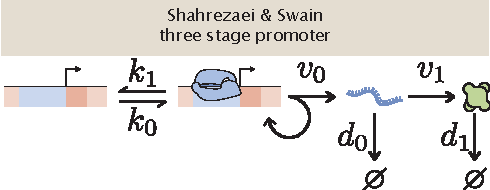
\includegraphics{../figures/si/figS0X_Shahrezaei_promoter.pdf}
\caption{\textbf{Schematic of three-stage promoter from~\cite{Shahrezaei2008}.}
Adapted from Shahrezaei \& Swain~\cite{Shahrezaei2008}. In their paper they
derive a closed form solution for the protein distribution. Our two-state bursty
promoter at the mRNA level can be mapped into their solution with some
relabeling.}
\label{fig:shahrezaei}
\end{figure}

To verify this intuitively conjectured mapping between our problem and the
solution in~\cite{Shahrezaei2008}, we continue with a careful solution for the
mRNA distribution using probability generating functions, following the ideas
sketched in~\cite{Shahrezaei2008}. It is natural to nondimensionalize rates in
the problem by $\gamma$, or equivalently, this amounts to measuring time in
units of $\gamma^{-1}$. We are also only interested in steady state, so we set
the time derivatives to zero, giving
\begin{align}
0 =& k_R^+ p_A(m) - k_R^- p_R(m) + (m+1) p_R(m+1) - m p_R(m)
\\
\begin{split}
0 =& - k_R^+ p_A(m) + k_R^- p_R(m) + (m+1) p_A(m+1) - m p_A(m) 
\\
&- k_i p_A(m) + k_i \sum_{m^\prime=0}^m \theta(1-\theta)^{m-m^\prime} p_A(m^\prime),
\end{split}
\end{align}
where for convenience we kept the same notation for all rates, but these are
now expressed in units of mean mRNA lifetime $\gamma^{-1}$.
        
The probability generating function is defined as before in the constitutive
case, except now we must introduce a generating function for each promoter
state,
\begin{align}
f_A(z) = \sum_{m=0}^\infty z^m p_A(m),
\;
f_R(z) = \sum_{m=0}^\infty z^m p_R(m).
\end{align}
Our real objective is the generating function $f(z)$ that generates the mRNA
distribution $p(m)$, independent of what state the promoter is in. But since
$p(m) = p_A(m) + p_R(m)$, it follows too that $f(z) = f_A(z) + f_R(z)$.

As before we multiply both equations by $z^m$ and sum over all $m$. Each
individual term transforms exactly as did an analogous term in the constitutive
case, so the coupled ODEs for the generating functions read
\begin{align}
0 =& k_R^+ f_A(z) - k_R^- f_R(z) + \pderiv{z} f_R(z) - z \pderiv{z} f_R(z)
\\
\begin{split}
0 =&  - k_R^+ f_A(z) + k_R^- f_R(z) + \pderiv{z} f_A(z) - z \pderiv{z} f_A(z)
\\
&- k_i f_A(z) + k_i \frac{\theta}{1-z(1-\theta)} f_A(z),
\end{split}
\end{align}
and after changing variables $\xi = 1 - \theta$ as before and rearranging, we
have
\begin{align}
0 &= k_R^+ f_A(z) - k_R^- f_R(z) + (1-z) \pderiv{z} f_R(z)
\\
0 &=  - k_R^+ f_A(z) + k_R^- f_R(z) + (1 - z) \pderiv{z} f_A(z)
+ k_i \frac{(z-1)\xi}{1-z\xi} f_A(z),
\end{align}
We can transform this problem from two coupled first-order ODEs to a single
second-order ODE by solving for $f_A$ in the first and plugging into the second,
giving
\begin{align}
\begin{split}
0 = (1&-z) \pderiv[f_R]{z}
+ \frac{1-z}{k_R^+}
        \left(k_R^- \pderiv[f_R]{z} + \pderiv[f_R]{z} +(z-1) \psecderiv[f_R]{z}\right)
\\
&+ \frac{k_i}{k_R^+} \frac{(z-1)\xi}{1-z\xi}
        \left(k_R^- f_R + (z-1) \pderiv[f_R]{z}\right),
\end{split}
\end{align}
where, to reduce notational clutter, we have dropped the explicit $z$ dependence
of $f_A$ and $f_R$. Simplifying we have
\begin{align}
0 = \psecderiv[f_R]{z}
        - \left(\frac{k_i\xi}{1-z\xi}
                + \frac{1 + k_R^- + k_R^+}{1-z}
        \right)\pderiv[f_R]{z}
        + \frac{k_i k_R^- \xi}{(1-z\xi)(1-z)}f_R.
\end{align}
This can be recognized as the hypergeometric differential equation, with
singularities at $z=1$, $z=\xi^{-1}$, and $z=\infty$. The latter can be verified
by a change of variables from $z$ to $x=1/z$, being careful with the chain rule,
and noting that $z=\infty$ is a singular point if and only if $x=1/z=0$ is a
singular point.

The standard form of the hypergeometric differential equation has its
singularities at 0, 1, and $\infty$, so to take advantage of the standard form
solutions to this ODE, we first need to transform variables to put it into a
standard form. However, this is subtle. While any such transformation should
work in principle, the solutions are expressed most simply in the neighborhood
of $z=0$, but the normalization condition that we need to enforce corresponds to
$z=1$. The easiest path, therefore, is to find a change of variables that maps 1
to 0, $\infty$ to $\infty$, and $\xi^{-1}$ to 1. This is most intuitively done
in two steps.

First map the $z=1$ singularity to 0 by the change of variables $v=z-1$, giving
\begin{align}
0 = \psecderiv[f_R]{v}
        + \left(\frac{k_i\xi}{(1+v)\xi - 1}
                + \frac{1 + k_R^- + k_R^+}{v}
        \right)\pderiv[f_R]{v}
        + \frac{k_i k_R^- \xi}{((1+v)\xi - 1)v}f_R.
\end{align}
Now two singularities are at $v=0$ and $v=\infty$. The third is determined by
$(1+v)\xi -1 = 0$, or $v=\xi^{-1} - 1$. We want another variable change that
maps this third singularity to 1 (without moving 0 or infinity). Changing
variables again to $w=\frac{v}{\xi^{-1} - 1} = \frac{\xi}{1-\xi} v$ fits the
bill. In other words, the combined change of variables
\begin{align}
w = \frac{\xi}{1-\xi} (z-1)
\end{align}
maps $z = \{1, \xi^{-1}, \infty\}$ to $w =\{0, 1, \infty\}$ as desired. Plugging
in, being mindful of the chain rule and noting
$(1 + v)\xi - 1 = (1 - \xi)(w - 1)$ gives
\begin{align}
0 = \left(\frac{\xi}{1-\xi}\right)^2 \psecderiv[f_R]{w}
+ \left(
        \frac{\xi k_i}{(1-\xi)(w-1)} + \frac{\xi(1 + k_R^- + k_R^+)}{(1-\xi)w}
\right) \frac{\xi}{1-\xi} \pderiv[f_R]{w}
+ \frac{k_i k_R^- \xi^2}{(1-\xi)^2 w(w-1)}f_R.
\end{align}
This is close to the standard form of the hypergeometric differential equation,
and some cancellation and rearrangement gives
\begin{align}
0 = w(w-1)\psecderiv[f_R]{w}
+ \left(k_i w + (1 + k_R^- + k_R^+)(w-1)\right) \pderiv[f_R]{w}
+ k_i k_R^- f_R.
\end{align}
and a little more algebra produces
\begin{align}
0 = w(1-w)\psecderiv[f_R]{w}
+ \left(1 + k_R^- + k_R^+
        - (1 + k_i + k_R^- + k_R^+)w
\right) \pderiv[f_R]{w}
- k_i k_R^- f_R,
\end{align}
which is the standard form. From this we can read off the solution in terms of
hypergeometric functions ${_2F_1}$ from any standard source,
e.g.~\cite{Abramowitz1964}, and identify the conventional parameters in terms of
our model parameters. We want the general solution in the neighborhood of $w=0$
($z=1$), which for a homogeneous linear second order ODE must be a sum of two
linearly independent solutions. More precisely, 
\mrm{the use of variable $\gamma$ here is confusing. Is it okay to change it to
$\delta$ or something else in order to avoid associating it with the mRNA
degradation rate?}
\begin{align}
f_R(w) = C_1 {_2F_1}(\alpha, \beta, \gamma; w)
+ C_2 w^{1-\gamma}{_2F_1}(1+\alpha-\gamma, 1+\beta-\gamma, 2-\gamma; w)
\end{align}
with parameters determined by
\begin{align}
\begin{split}
\alpha\beta &= k_i k_R^-
\\
1+\alpha+\beta &= 1+k_i+k_R^-+k_R^+
\\
\gamma &= 1 + k_R^- + k_R^+
\end{split}
\end{align}
and constants $C_1$ and $C_2$ to be set by boundary conditions. Solving for
$\alpha$ and $\beta$, we find
\footnote{
Note that $\alpha$ and $\beta$ are interchangeable in the definition of
${_2F_1}$ and differ only in the sign preceeding the radical.
}
\begin{align}
\begin{split}
\alpha &= \frac{1}{2}
\left(k_i+k_R^-+k_R^+ + \sqrt{(k_i+k_R^-+k_R^+)^2 - 4k_i k_R^-}\right)
\\
\beta &= \frac{1}{2}
\left(k_i+k_R^-+k_R^+ - \sqrt{(k_i+k_R^-+k_R^+)^2 - 4k_i k_R^-}\right)
\\
\gamma &= 1 + k_R^- + k_R^+.
\end{split}
\end{align}
Since the normalization condition requires that $f_R$ be finite at $w=0$,
we can immediately set $C_2=0$ to discard the second solution.
This is because all the rate constants are strictly positive,
so $\gamma>1$ and therefore $w^{1-\gamma}$ blows up as $w\rightarrow0$.
Now that we have $f_R$, we would like to find the generating function
for the mRNA distribution, $f(z) = f_A(z) + f_R(z)$.
We can recover $f_A$ from our solution for $f_R$, namely
\begin{align}
f_A(z) = \frac{1}{k_R^+}\left(k_R^- f_R(z) + (z-1) \pderiv[f_R]{z}\right)
\end{align}
or
\begin{align}
f_A(w) = \frac{1}{k_R^+}\left(k_R^- f_R(w) + w \pderiv[f_R]{w}\right),
\end{align}
where in the second line we transformed our original relation between
$f_R$ and $f_A$ to our new, more convenient, variable $w$.
Plugging our solution for $f_R(w) = C_1{_2F_1}(\alpha, \beta, \gamma; w)$
into $f_A$, we will require the differentiation rule for ${_2F_1}$,
which tells us
\begin{align}
\pderiv[f_R]{w} = C_1\frac{\alpha\beta}{\gamma}
                {_2F_1}(\alpha+1, \beta+1, \gamma+1; w),
\end{align}
from which it follows that
\begin{align}
f_A(w) = \frac{C_1}{k_R^+}
\left(
k_R^- {_2F_1}(\alpha, \beta, \gamma; w)
+ w\frac{\alpha\beta}{\gamma} {_2F_1}(\alpha+1, \beta+1, \gamma+1; w)
\right)
\end{align}
and therefore
\begin{align}
f(w) = C_1\left(1 + \frac{k_R^-}{k_R^+}\right)
        {_2F_1}(\alpha, \beta, \gamma; w)
+ w \frac{C_1}{k_R^+} \frac{\alpha\beta}{\gamma}
        {_2F_1}(\alpha+1, \beta+1, \gamma+1; w).
\end{align}
To proceed, we need one of the (many) useful identities known for
hypergeometric functions, in particular
\begin{align}
w\frac{\alpha\beta}{\gamma} {_2F_1}(\alpha+1, \beta+1, \gamma+1; w)
=
(\gamma-1)\left(
{_2F_1}(\alpha, \beta, \gamma-1; w) - {_2F_1}(\alpha, \beta, \gamma; w)
\right).
\end{align}
Substituting this for the second term in $f(w)$, we find
\begin{align}
f(w) = \frac{C_1}{k_R^+}
\left[
        \left(k_R^+ + k_R^-\right)
        {_2F_1}(\alpha, \beta, \gamma; w)
+ (\gamma-1)\left(
        {_2F_1}(\alpha, \beta, \gamma-1; w) - {_2F_1}(\alpha, \beta, \gamma; w)
        \right)
\right],
\end{align}
and since $\gamma-1 = k_R^+ + k_R^-$, the first and third terms cancel,
leaving only
\begin{align}
f(w) = C_1\frac{k_R^+ + k_R^-}{k_R^+} {_2F_1}(\alpha, \beta, \gamma-1; w).
\end{align}
Now we enforce normalization, demanding $f(w=0) = f(z=1) = 1$.
${_2F_1}(\alpha, \beta, \gamma-1; 0) = 1$, so we must have
$C_1 = k_R^+ / (k_R^+ + k_R^-)$ and consequently
\begin{align}
f(w) =  {_2F_1}(\alpha, \beta, k_R^+ + k_R^-; w).
\end{align}
Recalling that the mean burst size $b = (1-\theta)/\theta = \xi/(1-\xi)$
and $w = \frac{\xi}{1-\xi} (z-1) = b (z-1)$,
we can transform back to the original variable $z$ to find the tidy result
\begin{align}
f(z) =  {_2F_1}(\alpha, \beta, k_R^+ + k_R^-; b(z-1)),
\end{align}
with $\alpha$ and $\beta$ given above by
\begin{align}
\begin{split}
\alpha &= \frac{1}{2}
\left(k_i+k_R^-+k_R^+ + \sqrt{(k_i+k_R^-+k_R^+)^2 - 4k_i k_R^-}\right)
\\
\beta &= \frac{1}{2}
\left(k_i+k_R^-+k_R^+ - \sqrt{(k_i+k_R^-+k_R^+)^2 - 4k_i k_R^-}\right).
\end{split}
\end{align}
Finally we are in sight of the original goal. We can generate the steady-state
probability distribution of interest by differentiating the generating function,
\begin{align}
p(m) = m! \left.\frac{\partial^m}{\partial z^m} f(z) \right|_{z=0},
\end{align}
which follows easily from its definition. Some contemplation reveals that
repeated application of the derivative rule used above will produce products of
the form $\alpha(\alpha+1)(\alpha+2)\cdots(\alpha+m-1)$ in the expression for
$p(m)$ and similarly for $\beta$ and $\gamma$. These resemble ratios of
factorials, but since $\alpha$, $\beta$, and $\gamma$ are not necessarily
integer, we should express the ratios using gamma functions instead. More
precisely, one finds
\begin{align}
p(m) = \frac{
        \Gamma(\alpha + m)\Gamma(\beta + m)\Gamma(k_R^+ + k_R^-)
        }
        {
        \Gamma(\alpha)\Gamma(\beta)\Gamma(k_R^+ + k_R^- + m)
        }
\frac{b^m}{m!}{_2F_1}(\alpha+m, \beta+m, k_R^++k_R^-+m; -b)
\label{eq:p_m_bursty+rep_appdx}
\end{align}
which is finally the probability distribution we sought to derive.

\subsubsection{Moments of two-state bursty promoter mRNA distribution}

We can verify the correctness of~\eq{eq:p_m_bursty+rep_appdx} by comparison with
Gillespie simulation. We can also easily compute moments of the distribution
from the generating function, and check these against raw moments computed
directly from the master equation.

The $j$-th raw moment of the distribution can be computed from the generating
function from the formula
\begin{align}
\langle m^j \rangle
= \left. \left(z \frac{\partial}{\partial z}\right)^j f(z)\right|_{z=1}.
\end{align}
Note that \textit{probabilities} are generated by differentiating and evaluating
at $z=0$, while \textit{moments} are generated by differentiating and evaluating
at $z=1$. This also aligns with the normalization constraint, which can be
thought of as the zeroth raw moment.
        
The mean mRNA is given by
\begin{align}
\langle m \rangle = \left.z \pderiv[f]{z} \right|_{z=1}
= \frac{\alpha\beta b}{k_R^+ + k_R^-}
= k_i b\frac{k_R^-}{k_R^+ + k_R^-},
\end{align}
which is intuitive and appealingly simple: the mean mRNA is just the mean mRNA
in the absence of repression ($k_i b$, the burst rate time mean burst size)
times the fraction of time the repressor is bound, $k_R^-/(k_R^+ + k_R^-)$.

To compute the variance, let us first compute
\begin{align}
\begin{split}
\langle m^2\rangle
&= \left .z\pderiv{z}\left(z\pderiv[f]{z}\right) \right|_{z=1}
= \left. z\left(\pderiv[f]{z} + z\psecderiv[f]{z}\right)\right|_{z=1}
\\
&= \frac{\alpha\beta b}{k_R^+ + k_R^-}
        + \frac{\alpha(\alpha+1)\beta(\beta+1) b^2}
                {(k_R^+ + k_R^-)(k_R^+ + k_R^- + 1)}
\\
&= \frac{k_i b k_R^-}{k_R^+ + k_R^-}
        + \frac{k_i k_R^- b^2 (1 + k_i + k_R^+ + k_R^- + k_i k_R^-)}
                {(k_R^+ + k_R^-)(k_R^+ + k_R^- + 1)},
\end{split}
\end{align}
from which the variance is
\begin{align}
\begin{split}
var(m) = \langle m^2\rangle - \langle m\rangle^2
&= \frac{k_i b k_R^-}{k_R^+ + k_R^-}
\left(
1 + \frac{b(1 + k_i + k_R^+ + k_R^- + k_i k_R^-)} {k_R^+ + k_R^- + 1}
- \frac{k_i b k_R^-}{k_R^+ + k_R^-}
\right)
\\
&= k_i b\frac{k_R^-}{k_R^+ + k_R^-}
\left(
1 + b + k_i b\frac{1 + k_R^-} {k_R^+ + k_R^- + 1}
- \frac{k_i b k_R^-}{k_R^+ + k_R^-}
\right)
\\
&= k_i b\frac{k_R^-}{k_R^+ + k_R^-}
\left(
1 + b + k_i b\frac{k_R^+}{(k_R^+ + k_R^-)(k_R^+ + k_R^- + 1)}
\right).
\end{split}
\end{align}
The Fano factor is the quantity in parentheses. This can be interpreted as
the variability arising from the negative binomial distribution of the
unregulated promoter $(1+b)$ plus additional noise arising from repression.

\mmnote{Still to writeup: moment derivation direct from CME to compare}
\mrm{stopped reading here}

\subsection{Numerical considerations and recursion formulas}
\subsubsection{Generalities}
We would like to carry out Bayesian parameter inference on FISH data
from~\cite{Jones2014}, using~\eq{eq:p_m_bursty+rep_appdx} as our
likelihood. This requires accurate (and preferably fast)
numerical evaluation of the hypergeometric function ${_2F_1}$,
which is a notoriously hard problem~\cite{Pearson2017, Gil2007},
and our particular needs here present an especial challenge as we show below.

The hypergeometric function is defined by its Taylor series as
\begin{align}
{_2F_1}(a,b,c;z) 
= \sum_{l=0}^\infty
\frac{\Gamma(a + l)\Gamma(b + l)\Gamma(c)}
        {\Gamma(a)\Gamma(b)\Gamma(c + l)}
\frac{z^l}{l!}
\end{align}
for $|z|<1$, and by analytic continuation elsewhere.
If $z\lesssim1/2$ and $\alpha$ and $\beta$ are not too large
(absolute value below 20 or 30),
then the series converges quickly and an accurate numerical representation is
easily computed by truncating the series after a reasonable number of terms.
Unfortunately, we need to evaluate ${_2F_1}$ over mRNA copy numbers fully out
to the tail of the distribution, which can easily reach 50, possibly 100.
From~\eq{eq:p_m_bursty+rep_appdx}, this means evaluating ${_2F_1}$
repeatedly for values of $a$, $b$, and $c$ spanning the full range
from $\mathcal{O}(1)$ to $\mathcal{O}(10^2)$,
even if $\alpha$, $\beta$, and $\gamma$
in~\eq{eq:p_m_bursty+rep_appdx} are small,
with the situation even worse if they are not small.
A naive numerical evaluation of the series definition will be
prone to overflow and, if any of $a,b,c<0$, then some successive terms in the
series have alternating signs which can lead to catastrophic cancellations.

One solution is to evaluate ${_2F_1}$ using arbitrary precision arithmetic
instead of floating point arithmetic,
e.g., using the \texttt{mpmath} library in Python.
This is accurate but incredibly slow computationally.
To quantify how slow, we found that
evaluating the likelihood defined by~\eq{eq:p_m_bursty+rep_appdx} $\sim50$ times
(for a typical dataset of interest from~\cite{Jones2014},
with $m$ values spanning 0 to $\sim50$)
using arbitrary precision arithmetic is 100-1000 fold slower than
evaluating a negative binomial likelihood for the corresponding
constitutive promoter dataset.

To claw back $\gtrsim30$ fold of that slowdown, we can exploit
one of the many catalogued symmetries involving ${_2F_1}$.
The solution involves recursion relations originally explored by Gauss,
and studied extensively in~\cite{Pearson2017, Gil2007}.
They are sometimes known as contiguous relations and relate the values
of any set of 3 hypergeometric functions whose arguments differ by integers.
To rephrase this symbolically, consider a set of hypergeometric functions
indexed by an integer $n$,
\begin{align}
f_n = {_2F_1}(a+\epsilon_i n, b+\epsilon_j n, c+\epsilon_k n; z),
\end{align}
for a fixed choice of $\epsilon_i, \epsilon_j, \epsilon_k \in \{0,\pm 1\}$
(at least one of $\epsilon_i, \epsilon_j, \epsilon_k$ must be nonzero,
else the set of $f_n$ would contain only a single element).
Then there exist known recurrence relations of the form
\begin{align}
A_n f_{n-1} + B_n f_{n} + C_n f_{n+1} = 0,
\end{align}
where $A_n, B_n$, and $C_n$ are some functions of $a,b,c$, and $z$.
In other words, for fixed $\epsilon_i, \epsilon_j, \epsilon_k, a, b,$ and $c$,
if we can merely evaluate ${_2F_1}$ twice, say for $n^\prime$ and $n^\prime-1$,
then we can easily and rapidly generate values for arbitrary $n$.

This provides a convenient solution for our problem: we need repeated
evaluations of ${_2F_1}(a+m, b+m, c+m; z)$
for fixed $a,b$, and $c$ and many integer values of $m$.
They idea is that we can use arbitrary precision arithmetic to evaluate
${_2F_1}$ for just two particular values of $m$ and then generate
${_2F_1}$ for the other 50-100 values of $m$ using the recurrence
relation.\footnote{
There are even more sophisticated ways of utilizing the recurrence
relations that might have netted another factor of 2 speed-up, and
possibly as much as a factor of 10, but the method described here had
already reduced the computation time to an acceptable
$\mathcal{O}(\text{1 min})$, so these more sophisticated approaches did
not seem worth the time to pursue.
}

However, there two further wrinkles.
The first is that
a naive application of the recurrence relation is numerically unstable.
Roughly, this is because the three term recurrence relations,
like second order ODEs, admit two linearly independent solutions.
In a certain eigenbasis, one of these solutions dominates the other
as $n\rightarrow\infty$, and as $n\rightarrow-\infty$,
the dominance is reversed.
If we fail to work in this eigenbasis, our solution of the recurrence relation
will be a mixture of these solutions and rapidly accumulate numerical error.
For our purposes, it suffices to know that the authors of~\cite{Gil2007}
derived the numerically stable solutions (so-called \textit{minimal solutions})
for several possible choices of $\epsilon_i, \epsilon_j, \epsilon_k$.
Running the recurrence in the proper direction using a minimal solution
is numerically robust and can be done entirely in floating point arithmetic, 
so that we only need to evaluate ${_2F_1}$ with arbitrary precision arithmetic
to generate the seed values for the recursion.

The second wrinkle is a corollary to the first.
The minimal solutions are only minimal for certain ranges of the argument $z$,
and not all of the 26 possible recurrence relations
have minimal solutions for all $z$.
This can be solved by using one of the many transformation formulae for
${_2F_1}$ to convert to a different recurrence relation that has
a minimal solution over the required domain of $z$, although
this can require some trial and error to find the right transformation,
the right recurrence relation, and the right minimal solution.

\subsubsection{Particulars}
Let us now demonstrate these generalities for our problem of interest.
In order to evaluate the probability distribution of our
model,~\eq{eq:p_m_bursty+rep_appdx}, we need to evaluate hypergeometric functions
of the form ${_2F_1}(\alpha+m, \beta+m, \gamma+m; -b)$
for values of $m$ ranging from $0$ to $\mathcal{O}(100)$.
The authors of~\cite{Gil2007} did not derive a recursion relation
for precisely this case. We could follow their methods and do so ourselves,
but it is much easier to convert to a case that they did consider.
The strategy is to look through the minimal solutions tabulated
in~\cite{Gil2007} and search for a transformation we could apply to
${_2F_1}(\alpha+m, \beta+m, \gamma+m; -b)$ that would place the $m$'s
(the variable being incremented by the recursion)
in the same arguments of ${_2F_1}$ as the minimal solution.
After some ``guess and check,'' we found that the transformation
\begin{align}
{_2F_1}(\alpha+m, \beta+m, \gamma+m; -b)
=
(1+b)^{-\alpha-m}
        {_2F_1}\left(\alpha+m, \gamma-\beta, \gamma+m; \frac{b}{1+b}\right),
\label{eq:rec_euler_pretransform}
\end{align}
produces a ${_2F_1}$ on the right hand side that closely resembles
the minimal solutions $y_{3,m}$ and $y_{4,m}$ in Eq.~4.3 in~\cite{Gil2007}.
Explicitly, these solutions are
\begin{align}
y_{3,m}
&\propto
{_2F_1}\left(-\alpha^\prime + \gamma^\prime - m,
                -\beta^\prime + \gamma^\prime,
                1-\alpha^\prime-\beta^\prime+\gamma^\prime-m;
                1-z\right)
\\
y_{4,m}
&\propto
{_2F_1}\left(\alpha^\prime + m,
                \beta^\prime,
                1+\alpha^\prime+\beta^\prime-\gamma^\prime+m;
                1-z\right),
\label{eq:minimal_soln_sans_prefac}
\end{align}
where we have omitted prefactors which are unimportant for now.
Which of these two we should use depends on what values $z$ takes on.
Equating $1-z=b/(1+b)$ gives $z=1/(1+b)$, and since $b$ is strictly positive,
$z$ is bounded between 0 and 1.
From Eq.~4.5 in~\cite{Gil2007}, $y_{4,m}$ is the minimal solution
for real $z$ satisfying $0<z<2$, so this is the only minimal solution we need.

Now that we have our minimal solution,
what recurrence relation does it satisfy?
Confusingly, the recurrence relation of which $y_{4,m}$ is a solution
increments different arguments of ${_2F_1}$ that does $y_{4,m}$:
it increments the first only, rather than first and third.
This recurrence relation can be looked up, e.g., Eq.~15.2.10
in~\cite{Abramowitz1964}, which is
\begin{align}
(\gamma^\prime - (\alpha^\prime + m)) f_{m-1}
+
(2(\alpha^\prime+m) - \gamma^\prime + (\beta^\prime - \alpha^\prime)z)f_m
+ \alpha^\prime(z-1) f_{m+1} = 0.
\label{eq:chosen_rec_rel}
\end{align}
Now we must solve for the parameters appearing in the recurrence relation
in terms of our parameters, namely by setting
\begin{align}
\begin{split}
\alpha^\prime &= \alpha
\\
\beta^\prime &= \gamma - \beta
\\
1 + \alpha^\prime + \beta^\prime - \gamma^\prime &= \gamma
\\
1 - z &= \frac{b}{1+b}
\end{split}
\end{align}
and solving to find
\begin{align}
\begin{split}
\alpha^\prime &= \alpha
\\
\beta^\prime &= \gamma - \beta
\\
\gamma^\prime &= 1 + \alpha - \beta
\\
z &= \frac{1}{1+b}
.
\end{split}
\end{align}
Finally we have everything we need. The minimal solution
\begin{align}
y_{4,m}
=
\frac{\Gamma(1+\alpha^\prime-\gamma^\prime+m)}
        {\Gamma(1+\alpha^\prime+\beta^\prime-\gamma^\prime+m)}
\times
{_2F_1}\left(\alpha^\prime + m,
                \beta^\prime,
                1+\alpha^\prime+\beta^\prime-\gamma^\prime+m;
                1-z\right),
\end{align}
where we have now included the necessary prefactors,
is a numerically stable solution of the recurrence
relation~\eq{eq:chosen_rec_rel} if the recursion is run
from large $m$ to small $m$.
So the procedure is to compute the value of ${_2F_1}$ for the two
largest $m$ values of interest using arbitrary precision arithmetic,
compute the prefactors to construct
$y_{4,\text{max}(m)}$ and $y_{4,\text{max}(m)-1}$,
recursively compute $y_{4,m}$ for all $m$ less than $\text{max}(m)$ down
to $m=0$, then cancel off the prefactors of the resulting values of
$y_{4,m}$ for all $m$ to produce ${_2F_1}$ for all desired $m$ values.
\mmnote{Maybe I should reformat this paragraph into
a pseudocode version of the algorithm?
Instead of, or in addition to?}

With ${_2F_1}$ computed, the only remaining numerical danger in computing
$p(m)$ in~\eq{eq:p_m_bursty+rep_appdx} is overflow of the gamma functions.
This is easily solved by taking the log of the entire expression
and using standard routines to compute the log of the gamma functions,
then exponentiating the entire expression at the end if $p(m)$
is needed rather than $\log p(m)$.